\documentclass[11pt]{article}
\usepackage{../common/hypnos-paper}

\DeclareMathOperator{\BMO}{BMO}
\DeclareMathOperator{\dist}{dist}
\DeclareMathOperator{\sinc}{sinc}
\newcommand{\R}{\mathbb{R}}
\newcommand{\Z}{\mathbb{Z}}
\newcommand{\N}{\mathbb{N}}
\newcommand{\Lam}{\Lambda}
\newcommand{\E}{\mathcal{E}}

\hypnostitle{The unfolded zeros of the Riemann zeta function do not form a Riesz basis of exponentials}
\hypnosshorttitle{The unfolded zeta zeros are not a Riesz basis}
\hypnoswriter{Claude Fable 5.1 (Anthropic)}
\hypnosdate{September 29, 2026}

\begin{document}
\hypnosmaketitle

\begin{abstract}
Let $\gamma_1\le\gamma_2\le\cdots$ be the positive ordinates of the nontrivial zeros of $\zeta$, counted with multiplicity, and let $\theta$ be the Riemann--Siegel theta function. Unfold the ordinates to unit density by $x_n=\theta(\gamma_n)/\pi+3/2$, so that $x_n\approx n$, and for a real constant $a$ consider the symmetric sequences $\Lam_a=\{\pm(\theta(\gamma_n)/\pi+a)\}$, again with multiplicity; $\Lam_{3/2}\cup\{0\}$ is modeled on $\mathbb Z$ and $\Lam_1$ on $\mathbb Z+\tfrac12$. We prove three things about the exponential systems $\{e^{i\lambda t}:\lambda\in\Lam\}$ generated by these sequences. First, at every simple ordinate the displacement from the integer lattice is exactly the argument of zeta: $x_n-n=-S(\gamma_n)$ with $S(t)=\pi^{-1}\arg\zeta(\tfrac12+it)$ (at an ordinate, the mean of its one-sided limits). Second, Kadec's $1/4$ condition and Avdonin's ``$1/4$ in the mean'' condition fail unconditionally for every centering constant and every block length, although below height $T$ the block condition does hold at block lengths of order $\log^2 T$. Third, the main result: for every unfolding constant $a$ and every finite modification of $\Lam_a$, the system is not a Riesz basis for $L^2(I)$ for any bounded interval $I$. The obstruction is Selberg's theorem that the mean square of $S$ over $[T,2T]$ grows like $(2\pi^2)^{-1}\log\log T$: by the Hru\v{s}\v{c}ev--Nikol'skii--Pavlov characterization of exponential Riesz bases, a Riesz basis forces the deviation of the counting function from linearity into $\BMO(\R)$, and Selberg's variance growth is incompatible with bounded mean oscillation. No hypothesis on the zeros is assumed. The theorem concerns the sequence with multiplicity; for the set of distinct frequencies it is proved here only when all but finitely many ordinates are simple. The same argument applies to any $L$-function whose argument has a Selberg-type mean square and a bounded mean. By the Beurling--Malliavin theorem and Conrey's theorem that at least two fifths of the zeros are simple and on the critical line, the completeness radius of the set of distinct points lies between $2\pi/5$ and $\pi$ unconditionally, and equals $\pi$ if all but finitely many ordinates are simple; the exact unconditional completeness radius, the critical length, the frame property, and the separation of the positive half of $\Lam_a$ remain open. The questions and the numerical record that led to these theorems came from the Hypnos research harness and are reported in Section~\ref{sec:provenance}.
\end{abstract}

\begin{attribution}
This paper was written by Claude Fable 5.1, an AI model made by Anthropic, at the direction of David Ross. The model chose the problem from the record of Hypnos, the research harness described in Section~\ref{sec:provenance}, proved the theorems, wrote the verification programs and the text; David Ross set the task, ran the process, and takes responsibility for the manuscript. Four reviews were applied, each with a per-item ledger. On 2026-09-29, Claude Opus 5.5 (Anthropic, a model other than the writer), in a fresh context, found no blocking error and five major items; GPT-6 Astra (OpenAI), through the Codex CLI, found one blocking error (a completeness statement that counted ordinates with multiplicity where completeness depends only on the set of distinct points; since restated) and five major items. A further review by GPT-6 Astra, completed on October 1, 2026 (EDT), found two major items (a finite-height necessity claim the proof did not cover; the lower bound for the distinct ordinates that Conrey's theorem supplies, which the paper had denied) and four minor ones, and comments from a separate Claude Opus 5.5 session of October 1 found the Conrey bound and an overclaim in Section~\ref{sec:provenance}. A final review by Claude Opus 5.5 on October 2 found no blocking error, one major item outside the manuscript (its README) and nine minor ones. All of these were applied. The reviews and the per-item dispositions accompany the source. David Ross read every page, for the only things he can judge: that the account of the harness and of the process matches the record, and that nothing reads like a machine grading its own homework. He did not check the proofs, and could not have; a reader should take his reading as a check for red flags, not as a review. No human mathematician has reviewed this paper. It is one of three manuscripts written from the Hypnos record on the night of 2026-09-28/29, after Astra's paper on approximate antiunitary symmetry and before the note on Gil's questions; it was written without reading the other two.
\end{attribution}

\section{Introduction}

This paper studies exponential systems whose frequencies are the symmetrized, unfolded ordinates of the nontrivial zeros of the Riemann zeta function. A real sequence $\Lam$ generates the exponential system $\E(\Lam)=\{e^{i\lambda t}:\lambda\in\Lam\}$, and one asks whether $\E(\Lam)$ is complete, a frame, or a Riesz basis in $L^2(I)$ for an interval $I$; equivalently, whether $\Lam$ is a uniqueness set, a sampling set, or a complete interpolating sequence for the Paley--Wiener space of band-limited functions. The classical theory (Paley--Wiener, Levinson, Kadec, Avdonin, Beurling--Malliavin, Pavlov) answers such questions in terms of the counting function of $\Lam$.

The ordinates $\gamma_n$ themselves have density $\frac{1}{2\pi}\log\frac{t}{2\pi}$ at height $t$, which tends to infinity, so they cannot generate a Riesz basis or a frame for any interval. The natural object is the \emph{unfolded} sequence. With $\theta$ the Riemann--Siegel theta function we put
\begin{equation}\label{eq:unfold}
x_n=\frac{\theta(\gamma_n)}{\pi}+\frac32\qquad(n\ge1),\qquad \Lam_a=\{\theta(\gamma_n)/\pi+a:n\ge1\}\cup\{-\theta(\gamma_n)/\pi-a:n\ge1\}\quad(a\in\R),
\end{equation}
sequences counted with multiplicity. The constant $\frac32$ makes $x_n\approx n$ (Theorem~\ref{thm:identity}), so $\Lam_{3/2}\cup\{0\}$ is a symmetric perturbation of $\Z$ and $\Lam_1$ a symmetric perturbation of $\Z+\frac12$, both of density one; we ask about $\E(\Lam_a)$ on $L^2(-\pi,\pi)$, the interval matched to that density. Note that changing $a$ moves the two halves of $\Lam_a$ in opposite directions, so it is not a translation; that is why the main theorem is stated for every $a$. We write $\Lam=\Lam_{3/2}$ when the constant is not at issue.

The results are as follows. Section~\ref{sec:identity} shows that the unfolding \eqref{eq:unfold} is exactly the one for which the displacement from the lattice is the argument of zeta, $x_n-n=-S(\gamma_n)$ at every simple ordinate, and that sums of displacements over blocks are governed by $\int\theta' S$ and by jumps of $S^2/2$ (Theorem~\ref{thm:identity}, Proposition~\ref{prop:block}). Section~\ref{sec:kadec} shows that Kadec's uniform condition and Avdonin's averaged condition both fail, for every centering and every fixed block length, as an unconditional consequence of the unboundedness of $S$ (Theorem~\ref{thm:kadec}); a companion estimate shows that below height $T$ the averaged condition holds once the block length is of order $\log^2 T$ (Corollary~\ref{cor:growing}), so the failure is slow: on the harness's table of the first $10^5$ ordinates the averaged condition holds at every tested block length from $8$ upward (Section~\ref{sec:numerics}), while no block length survives at all heights. Section~\ref{sec:main} proves the main theorem: for every unfolding constant $a$ and every finite modification $\Lam'$ of $\Lam_a$, $\E(\Lam')$ is not a Riesz basis for $L^2(I)$ for any bounded interval $I$ (Theorem~\ref{thm:main}). The proof combines the Hru\v{s}\v{c}ev--Nikol'skii--Pavlov form of Pavlov's theorem, which makes bounded mean oscillation of $n_\Lam(x)-x$ necessary, with Selberg's mean-square theorem for $S$ and Littlewood's bound for $\int S$; the mechanism is general (Theorem~\ref{thm:general}) and applies to $L$-functions with a Selberg-type argument variance (Corollary~\ref{cor:L}). Section~\ref{sec:survives} records what survives: the completeness radius of the set of distinct points lies between $2\pi/5$ and $\pi$ unconditionally, and equals $\pi$ if all but finitely many ordinates are simple (Theorem~\ref{thm:BM}); finite sections of the Gram matrix obey a pair bound consistent with the observed decay of the lower Riesz constant (Proposition~\ref{prop:finite}); and the exact unconditional completeness radius, the critical length, the frame property, and separation remain open (Section~\ref{sec:open}). Section~\ref{sec:numerics} reports the numerical record, and Section~\ref{sec:provenance} the provenance of the problem.

The obstruction in Theorem~\ref{thm:main} is worth stating in words. A Riesz basis of exponentials can tolerate certain unbounded displacements from the lattice: Pavlov's criterion shows that the sequence $n+c\log(2+|n|)$ generates a Riesz basis of $L^2(-\pi,\pi)$ for every $|c|\le1$ (Remark~\ref{rem:drift} sketches the verification). What it does not tolerate is displacement whose local variance grows without bound. Selberg's central limit theorem says that $S(t)$, for $t\in[T,2T]$, is asymptotically Gaussian with variance $(2\pi^2)^{-1}\log\log T$; the theorem below is the statement that this variance growth, together with the counting formula and the bounded mean of $S$, already forbids a Riesz basis.

\section{Classical inputs}\label{sec:inputs}

\subsection{The argument of zeta}
For $t>0$ not an ordinate let $N(t)$ be the number of zeros $\rho=\beta+i\gamma$ of $\zeta$ with $0<\gamma\le t$, counted with multiplicity. The Riemann--von Mangoldt formula reads
\begin{equation}\label{eq:RvM}
N(t)=\frac{\theta(t)}{\pi}+1+S(t),\qquad S(t)=\frac1\pi\arg\zeta(\tfrac12+it),
\end{equation}
where the argument is obtained by continuous variation along the segments from $2$ to $2+it$ and from $2+it$ to $\frac12+it$, and
\[
\theta(t)=\arg\Gamma(\tfrac14+\tfrac{it}{2})-\frac t2\log\pi=\frac t2\log\frac{t}{2\pi}-\frac t2-\frac\pi8+\frac1{48t}+O(t^{-3}).
\]
At an ordinate $\gamma$ we define $S(\gamma)$ and $N(\gamma)$ as the means of the one-sided limits; then \eqref{eq:RvM} holds for every $t>0$. Three facts about $\theta$ and $S$ are used throughout: $\theta$ is real analytic with $\theta'(t)=\frac12\log\frac{t}{2\pi}+O(t^{-2})$, hence strictly increasing on $[7,\infty)$; on $[7,\infty)$, between consecutive ordinates, $S(t)=N(t)-\theta(t)/\pi-1$ is strictly decreasing; and at an ordinate of multiplicity $m$ the function $S$ jumps by $+m$. Here the \emph{multiplicity of an ordinate} $\gamma$ is the total jump $m$ of $N$ at $\gamma$, the number of zeros $\beta+i\gamma$ with that ordinate counted with their multiplicities, and the ordinate is \emph{simple} if $m=1$. A simple ordinate carries one simple zero; a simple zero need not lie on a simple ordinate, since two simple zeros $\beta+i\gamma$ and $1-\beta+i\gamma$ share an ordinate. Under the Riemann hypothesis the two notions coincide. The $10^5$ ordinates in the table used in Section~\ref{sec:numerics} are distinct and belong to simple zeros on the critical line.

We use four classical theorems.
\begin{enumerate}
\item[(S1)] (Selberg \cite{Selberg46}) $\displaystyle\int_T^{2T}S(t)^2\,dt=\frac{T}{2\pi^2}\log\log T+O\bigl(T(\log\log T)^{1/2}\bigr)$.
\item[(S2)] (Littlewood \cite{Littlewood24}; \cite[Theorem 9.9(A)]{Titchmarsh}) $S_1(T)=\int_0^T S(t)\,dt=O(\log T)$.
\item[(S3)] (Selberg \cite{Selberg46}; see also Tsang \cite{Tsang86}) $S(t)=\Omega_\pm\bigl((\log t)^{1/3}(\log\log t)^{-7/3}\bigr)$; in particular $S$ is unbounded above and unbounded below.
\item[(S4)] (\cite[Theorem 9.4]{Titchmarsh}) $S(t)=O(\log t)$.
\end{enumerate}
All four are unconditional. Under the Riemann hypothesis the bounds in (S2) and (S4) improve to $O(\log T/(\log\log T)^2)$ and $O(\log t/\log\log t)$, both due to Littlewood \cite{Littlewood24} (Goldston and Gonek \cite{GoldstonGonek} give the constant $\frac12$ in the second); nothing below assumes the hypothesis.

\subsection{Exponential bases}
Let $I\subset\R$ be a bounded interval. The system $\E(\Lam)$ is a \emph{Riesz basis} for $L^2(I)$ if it is the image of an orthonormal basis under a bounded invertible operator; equivalently, it is complete and there are constants $0<A\le B$ with $A\sum|c_\lambda|^2\le\|\sum c_\lambda e^{i\lambda t}\|_{L^2(I)}^2\le B\sum|c_\lambda|^2$ for all finite sums. For $I=(-\pi,\pi)$ this is the same as $\Lam$ being a complete interpolating sequence for the Paley--Wiener space $PW_\pi$ of entire functions of exponential type at most $\pi$ that are square integrable on $\R$.

\begin{theorem}[Kadec \cite{Kadec64}]\label{thm:Kadec}
If $\Lam=\{\lambda_n\}_{n\in\Z}\subset\R$ and $\sup_n|\lambda_n-n|<\frac14$, then $\E(\Lam)$ is a Riesz basis for $L^2(-\pi,\pi)$. The constant $\frac14$ cannot be replaced by a larger one.
\end{theorem}

\begin{theorem}[Avdonin \cite{Avdonin74}; see \cite{AlemanyNitzan} for the form used here]\label{thm:Avdonin}
Let $\lambda_n=n+\delta_n$ ($n\in\Z$) be real and suppose
\begin{enumerate}
\item[(a)] $\inf_{n\ne m}|\lambda_n-\lambda_m|>0$,
\item[(b)] $\sup_n|\delta_n|<\infty$,
\item[(c)] there are $c\in\R$, $N\in\N$ and $d<\frac14$ with $\displaystyle\Bigl|\frac1N\sum_{n=mN+1}^{(m+1)N}\delta_n-c\Bigr|\le d$ for every $m\in\Z$.
\end{enumerate}
Then $\E(\Lam)$ is a Riesz basis for $L^2(-\pi,\pi)$.
\end{theorem}

Condition (c) is stated over the fixed partition of $\Z$ into blocks of length $N$; the statement in \cite{AlemanyNitzan} has $c=0$ and the blocks $mN\le n<(m+1)N$, and the centering constant and this offset are harmless because a common shift of all frequencies is a modulation. The sliding-window form (the same bound for every block of $N$ consecutive indices) is a stronger hypothesis; Theorem~\ref{thm:kadec} shows that both forms fail.

The complete description is due to Pavlov \cite{Pavlov79}, in the form given by Hru\v{s}\v{c}ev, Nikol'skii and Pavlov \cite[p.~240]{HNP}; we quote it as stated by Kozma and Lev \cite[Theorem 5.1]{KozmaLev}, translated from their normalization $\{e^{2\pi i\lambda t}\}$ on $(0,a)$ to ours. For a real sequence $\Lam$ the counting function $n_\Lam$ is defined up to an additive constant by $n_\Lam(b)-n_\Lam(a)=\#(\Lam\cap[a,b))$ for $a<b$. A locally integrable $f$ on $\R$ has bounded mean oscillation, $f\in\BMO(\R)$, if $\sup_J|J|^{-1}\int_J|f-f_J|\,dx<\infty$ over all bounded intervals $J$, where $f_J$ is the mean of $f$ on $J$.

\begin{theorem}[Pavlov; Hru\v{s}\v{c}ev--Nikol'skii--Pavlov]\label{thm:HNP}
Let $\Lam\subset\R$. Then $\E(\Lam)$ is a Riesz basis for $L^2(-\pi,\pi)$ if and only if
\begin{enumerate}
\item[(i)] $\Lam$ is separated: $\inf\{|\lambda-\mu|:\lambda\ne\mu\in\Lam\}>0$;
\item[(ii)] $f(x)=n_\Lam(x)-x$ belongs to $\BMO(\R)$;
\item[(iii)] for some $y>0$ the harmonic extension $U_f(x+iy)$ of $f$ to the upper half plane can be written on $\R$ as $c+\tilde u(x)+v(x)$ with $c$ constant, $u,v\in L^\infty(\R)$, $\|v\|_\infty<\frac14$, and $\tilde u$ the Hilbert transform of $u$.
\end{enumerate}
\end{theorem}

Only the necessity of (ii) is used below. Two further classical facts: by the John--Nirenberg inequality \cite{JohnNirenberg}, $f\in\BMO(\R)$ implies $\sup_J|J|^{-1}\int_J|f-f_J|^2\,dx<\infty$; and by Landau's theorem \cite{Landau67}, if $\E(\Lam)$ is a Riesz basis for $L^2(I)$ then $\Lam$ has uniform density $|I|/2\pi$, that is, $n_\Lam(x)=\frac{|I|}{2\pi}x+o(x)$ in the strong sense that the lower and upper Beurling densities both equal $|I|/2\pi$. Finally, the Beurling--Malliavin theorem \cite{BM67,KoosisII} states that the radius of completeness $R(\Lam)=\sup\{a:\E(\Lam)\text{ is complete in }L^2(-a,a)\}$ equals $\pi D_{BM}(\Lam)$, where the exterior Beurling--Malliavin density $D_{BM}(\Lam)$ is the supremum of the numbers $d$ for which there is a ``long'' family of disjoint intervals $\{I_k\}$, $\sum_k|I_k|^2/(1+\dist(0,I_k)^2)=\infty$, with $\#(\Lam\cap I_k)\ge d|I_k|$ for every $k$.

\section{The unfolding and the displacement identity}\label{sec:identity}

Since $\gamma_1=14.13\ldots>7$ and $\theta$ is increasing on $[7,\infty)$, the sequence $(x_n)$ of \eqref{eq:unfold} is nondecreasing, strictly increasing across distinct ordinates ($x_n<x_{n+1}$ exactly when $\gamma_n<\gamma_{n+1}$), and $x_1=0.9497\ldots$. Write $d_n=x_n-n$ for the displacement.

\begin{theorem}\label{thm:identity}
Let $\gamma_n=\gamma$ have multiplicity $m$ and write $n=N(\gamma^-)+j$ with $1\le j\le m$, where $N(\gamma^-)$ is the number of ordinates below $\gamma$. Then
\[
x_n-n=-S(\gamma)+\frac{m+1}{2}-j .
\]
In particular, if the ordinate $\gamma_n$ is simple then $x_n-n=-S(\gamma_n)$.
\end{theorem}

\begin{proof}
With the mean-value convention, $N(\gamma)=N(\gamma^-)+m/2=n-j+m/2$. By \eqref{eq:RvM}, $S(\gamma)=N(\gamma)-\theta(\gamma)/\pi-1=(n-j+m/2)-(x_n-3/2)-1$, which rearranges to the claim.
\end{proof}

Thus the constant $\frac32$ in \eqref{eq:unfold} is the unique unfolding constant for which the displacement is exactly $-S(\gamma_n)$ at simple ordinates. For the one-sided sequence $(x_n)$ another constant is a translation of all frequencies, harmless for basis questions (multiplication of $L^2(I)$ by $e^{ict}$ is unitary) but shifting every numerical threshold. For the symmetric sequences $\Lam_a$ it is not: $\Lam_{3/2}\cup\{0\}$ is the perturbation $\{0\}\cup\{\pm(n+d_n)\}$ of $\Z$, while $\Lam_1$ is the perturbation $\{\pm(n-\frac12+d_n)\}$ of $\Z+\frac12$, and $\Lam_{3/2}$ itself is a perturbation of $\Z\setminus\{0\}$, which is deficient by one point. On the table of Section~\ref{sec:numerics}, where every ordinate is simple, the multiplicity correction vanishes; the general form matters only for the statements.

\begin{proposition}\label{prop:block}
Let $7\le a<b$ be real numbers that are not ordinates. Then
\begin{equation}\label{eq:block}
\sum_{a<\gamma<b}S(\gamma)=\frac1\pi\int_a^b\theta'(t)S(t)\,dt+\frac{S(b)^2-S(a)^2}{2},
\end{equation}
the sum running over the ordinates in $(a,b)$ counted with multiplicity. Consequently, if the ordinates in $(a,b)$ are exactly $\gamma_{k+1},\dots,\gamma_{k+M}$ (with multiplicity),
\begin{equation}\label{eq:blockd}
\sum_{n=k+1}^{k+M}d_n=-\frac1\pi\int_a^b\theta'(t)S(t)\,dt-\frac{S(b)^2-S(a)^2}{2}.
\end{equation}
\end{proposition}

\begin{proof}
On an open interval free of ordinates, $S$ is continuously differentiable with $S'=-\theta'/\pi$, so $\pi^{-1}\theta'S=-SS'=-(S^2/2)'$. Hence $F(t)=\pi^{-1}\int_7^t\theta'S\,du+S(t)^2/2$ is constant on every such interval, and at an ordinate $\gamma$ of multiplicity $m$ it jumps by $\frac12\bigl(S(\gamma^+)^2-S(\gamma^-)^2\bigr)=\frac12\bigl(S(\gamma^+)-S(\gamma^-)\bigr)\bigl(S(\gamma^+)+S(\gamma^-)\bigr)=mS(\gamma)$. Therefore $F(b)-F(a)=\sum_{a<\gamma<b}m(\gamma)S(\gamma)$, which is \eqref{eq:block}. For \eqref{eq:blockd}, Theorem~\ref{thm:identity} gives $d_n=-S(\gamma)+\frac{m+1}{2}-j$ over the $m$ indices $n$ belonging to an ordinate $\gamma$ of multiplicity $m$, and the corrections $\frac{m+1}{2}-j$, $1\le j\le m$, sum to zero.
\end{proof}

The counting function of $\Lam_a$ is also the argument of zeta, in a changed variable. Fix $a\in\R$ and let $x_a(t)=\theta(t)/\pi+a$, so that the points of $\Lam_a$ are $\pm x_a(\gamma_n)$. For negative $a$ finitely many $x_a(\gamma_n)$ are negative and their reflections are positive, the largest of them being $-x_a(\gamma_1)$; the cutoff below is chosen past all of them. Let $X_a>\max\{1,\,x_a(7),\,-x_a(\gamma_1)\}$ be a number that is not a point of $\Lam_a$, and for $x\ge X_a$ let $t_a(x)\ge7$ be defined by $x_a(t_a(x))=x$; the map $x\mapsto t_a(x)$ is an increasing bijection of $[X_a,\infty)$ onto $[t_a(X_a),\infty)$ with $dt/dx=\pi/\theta'(t)$, and $t_a(X_a)$ is not an ordinate. Counting functions of sequences are taken with multiplicity.

\begin{lemma}\label{lem:counting}
For $x\ge X_a$ such that $t_a(x)$ is not an ordinate, $n_{\Lam_a}(x)-x=S(t_a(x))+c_0$, where $c_0$ is a constant depending only on $a$, on $X_a$ and on the normalization of $n_{\Lam_a}$. If $\Lam'$ is a finite modification of $\Lam_a$ then $n_{\Lam'}(x)-x=S(t_a(x))+c_0+b(x)$ with $b$ bounded and constant beyond the last modified point.
\end{lemma}

\begin{proof}
For $x\ge X_a$ the points of $\Lam_a$ in $[X_a,x)$ are the $x_a(\gamma_n)$ with $X_a\le x_a(\gamma_n)<x$, since every reflected point $-x_a(\gamma_n)$ is either negative or at most $-x_a(\gamma_1)<X_a$. Because $\theta$ is increasing on $[7,\infty)$ and $\gamma_1>7$, the condition $X_a\le x_a(\gamma_n)<x$ is the condition $t_a(X_a)\le\gamma_n<t_a(x)$, so $n_{\Lam_a}(x)-n_{\Lam_a}(X_a)=N(t_a(x))-N(t_a(X_a))$ when $t_a(x)$ is not an ordinate. By \eqref{eq:RvM} with $t=t_a(x)$ and the definition of $t_a$, $n_{\Lam_a}(x)-x=\theta(t)/\pi+1+S(t)-\theta(t)/\pi-a+n_{\Lam_a}(X_a)-N(t_a(X_a))=S(t_a(x))+c_0$. A finite modification changes the counting function by a bounded function that is constant beyond the last added or removed point.
\end{proof}

\section{Kadec and Avdonin fail for every block length}\label{sec:kadec}

\begin{theorem}\label{thm:kadec}
For every $N\ge1$ and every $c\in\R$,
\[
\sup_{k\ge0}\Bigl(\frac1N\sum_{n=k+1}^{k+N}d_n-c\Bigr)=+\infty
\qquad\text{and}\qquad
\inf_{k\ge0}\Bigl(\frac1N\sum_{n=k+1}^{k+N}d_n-c\Bigr)=-\infty .
\]
The same holds with $k$ restricted to the multiples of $N$, that is, along the fixed partition of the indices into blocks of length $N$. In particular $\sup_n|x_n-n-c|=\infty$ for every $c$ (the case $N=1$), so the hypothesis of Kadec's theorem fails for every centering, and hypotheses (b) and (c) of Avdonin's theorem fail for every centering and every block length, in the partition form as well as in the sliding-window form. The statements transfer to the symmetric sequence $\Lam_{3/2}\cup\{0\}$, whose displacements from $\Z$ are $\pm d_n$, and to $\Lam_1$ relative to $\Z+\frac12$.
\end{theorem}

\begin{proof}
Fix $N$ and $c$ and let $A>0$. By (S3) there is $t\ge\gamma_{2N}$ with $S(t)\ge A+1$; since $S(\gamma^+)\ge S(\gamma)$ at ordinates and $S$ is continuous on the open intervals between them, there is a non-ordinate $t_0\ge\gamma_{2N}$ with $S(t_0)\ge A$. Let $k+1\le n\le k+N$ be any block of $N$ consecutive indices with $k+N\le N(t_0)$ and $k+1\ge N(t_0)-2N+1$; the block $k=N(t_0)-N$ of the $N$ largest ordinates below $t_0$ qualifies, and so does the last block of the fixed partition ending at or below $N(t_0)$. For such $n$ we have $\theta(\gamma_n)\le\theta(t_0)$, and by \eqref{eq:RvM} at $t_0$,
\[
d_n=\frac{\theta(\gamma_n)}{\pi}+\frac32-n\le\frac{\theta(t_0)}{\pi}+\frac32-n=N(t_0)-1-S(t_0)+\frac32-n\le\bigl(N(t_0)-n\bigr)+\frac12-A ,
\]
and $N(t_0)-n\le2N-1$, so $\frac1N\sum_{n=k+1}^{k+N}d_n-c\le2N-\frac12-A-c$; for the block $k=N(t_0)-N$ the exact average of $N(t_0)-n$ is $\frac{N-1}{2}$ and the bound improves to $\frac N2-A-c$. As $A$ was arbitrary this gives the infimum. For the supremum choose a non-ordinate $t_0$ with $S(t_0)\le-A$ and a block with $k\ge N(t_0)$ and $k+N\le N(t_0)+2N$ (the $N$ smallest ordinates above $t_0$, or the first partition block starting above $N(t_0)$), and use $\theta(\gamma_n)\ge\theta(t_0)$: $d_n\ge N(t_0)-1-S(t_0)+\frac32-n\ge A+\frac12-2N$.
\end{proof}

The proof uses only the monotonicity of $\theta$ and of $N$ and the unboundedness of $S$ in both directions. It says more than the theorem states. The $N$ displacements just before a positive excursion $S(t_0)=A$ average at most $\frac N2-A$, so the sliding window of the $N$ ordinates preceding the excursion has mean below $-\frac14$ as soon as $A>\frac N2+\frac14$; the last complete block of the fixed partition, which ends $r=N(t_0)\bmod N$ indices earlier, has mean at most $r+\frac N2-A$ and needs $A>r+\frac N2+\frac14$; for centered means these thresholds decrease by $c$, and at a negative excursion $S(t_0)=-A$ the following window has mean at least $A-\frac N2$, with threshold $A>\frac N2+\frac14+c$. An excursion defeats the windows named here, not every window of that length. The next statement bounds how long a block must be for the mean to come back under control.

\begin{corollary}\label{cor:growing}
There is an absolute constant $C$ such that for all non-ordinates $7\le a<b$,
\[
\Bigl|\sum_{a<\gamma<b}S(\gamma)\Bigr|\le C\log^2 b .
\]
Hence, with a larger absolute constant $C$, for every block of $M$ consecutive indices whose ordinates lie below height $b$, $\bigl|\frac1M\sum d_n\bigr|\le C\log^2 b/M$, which is below $\frac14$ as soon as $M>4C\log^2b$. Under the Riemann hypothesis $\log^2b$ may be replaced by $\log^2 b/(\log\log b)^2$.
\end{corollary}

\begin{proof}
Integrate by parts in \eqref{eq:block}: $\int_a^b\theta'S\,dt=\theta'(b)S_1(b)-\theta'(a)S_1(a)-\int_a^b\theta''(t)S_1(t)\,dt$ with $\theta'(t)=O(\log t)$, $\theta''(t)=O(1/t)$ and $S_1(t)=O(\log t)$ by (S2); the two boundary terms are $O(\log^2b)$ and the integral is $O(\log b\cdot\log(b/a))$. The terms $S(a)^2,S(b)^2$ in \eqref{eq:block} are $O(\log^2b)$ by (S4). For the block statement, \eqref{eq:blockd} applies to blocks made of complete ordinate clusters; a block of indices that cuts through an ordinate of multiplicity $m$ differs from one that does not by at most $m$ displacements, each $O(\log b)$ by Theorem~\ref{thm:identity} and (S4), and $m=O(\log b)$, so the correction is $O(\log^2b)$ and is absorbed into $C$. The conditional statement uses the conditional forms of (S2) and (S4).
\end{proof}

Theorem~\ref{thm:kadec} and Corollary~\ref{cor:growing} bracket, for the uncentered sliding-window form, the block length at which the averaged condition holds for the windows below height $T$: a positive excursion $S(t_0)=A$ at a non-ordinate $t_0\le T$ with at least $N$ ordinates below it defeats the window of the $N$ ordinates preceding it unless $N>2A-\frac12$, so the block length must exceed $2A-\frac12$ for every such excursion (a negative excursion defeats the window that follows it, which may lie above $T$, so it is not counted here), and by Corollary~\ref{cor:growing} a length $C\log^2T$ suffices. This is a statement at a given height; Avdonin's hypothesis asks for one block length at all heights, and Theorem~\ref{thm:kadec} says that no such length exists. Since $\max|S(t)|$ over the harness's table, whose last ordinate lies at height $7.49\cdot10^4$, is about $1.63$, the mechanism, which needs an excursion of $S$ above $\frac N2+\frac14$ to defeat a window of length $N$, does not bite on that table for any $N\ge3$; the largest value of $|S|$ in the published record known to us, $S\approx3.3455$ just after a zero near $t=7.7573\cdot10^{27}$ in the computation of Bober and Hiary \cite[Table 2]{Bober}, defeats every $N\le6$, while $N=8$, the smallest tested block length on which the harness's table satisfied the $\frac14$ bound, needs an excursion above $4.25$, larger than any value of $S$ we know to have been computed. The numerical block means in Section~\ref{sec:numerics} decay approximately like $M^{-1}$ over the tested range, as \eqref{eq:blockd} predicts at heights where $S_1$ and $S^2$ are $O(1)$.

\section{No Riesz basis}\label{sec:main}

\begin{theorem}\label{thm:main}
Let $a\in\R$, let $\Lam_a$ be the unfolded zero sequence \eqref{eq:unfold}, and let $\Lam'$ be any finite modification of $\Lam_a$ (finitely many points added or removed, counted with multiplicity). For every bounded interval $I\subset\R$ and every $c\in\R$, the system $\{e^{i\lambda t}:\lambda\in\Lam'+c\}$ is not a Riesz basis for $L^2(I)$. In particular this holds for $\Lam_{3/2}\cup\{0\}$, for $\Lam_1$, and for $\Lam_{3/2}$. The same holds for the one-sided system $\{e^{ix_nt}:n\ge1\}$.
\end{theorem}

A Riesz basis has no repeated element, so if $\Lam'$ contains a repeated frequency the conclusion holds trivially, and the content of the theorem is the case of distinct frequencies, in which $n_{\Lam'}$ is the ordinary counting function of a set. Repeated frequencies in $\Lam_a$ come from ordinates of multiplicity $m\ge2$, each contributing $m$ copies of $x_a(\gamma)$ and of its reflection, and from the finitely many coincidences $x_a(\gamma_n)=-x_a(\gamma_m)$ between the two halves (these require $\theta(\gamma_n)+\theta(\gamma_m)=-2\pi a$, and $\theta(\gamma_n)\to\infty$). Finitely many repetitions can be removed by a finite modification, which changes the counting function by a bounded function; infinitely many cannot. So the theorem holds for every sequence $\Lam'$ as stated, and for the set of distinct points of $\Lam_a$ it is proved whenever all but finitely many ordinates are simple; without that hypothesis the counting function of the set is not controlled by Lemma~\ref{lem:counting}, and the theorem says nothing about it.

\begin{proof}
Translating $\Lam'$ by $c$ multiplies each element by the unimodular function $e^{ict}$, a unitary operator on $L^2(I)$, and translating $I$ multiplies each element by a unimodular constant; neither affects the Riesz basis property, so we may take $c=0$ and $I$ centered at $0$.

By Lemma~\ref{lem:counting} and (S4), $n_{\Lam'}(x)-n_{\Lam'}(0)=x+O(\log x)$ as $x\to+\infty$. Landau's theorem \cite{Landau67} says that a sampling sequence for $PW_{|I|/2}$ has lower Beurling density at least $|I|/2\pi$ and an interpolating sequence has upper Beurling density at most $|I|/2\pi$; a Riesz basis for $L^2(I)$ is both. Since the windows $[0,x]$ alone give $D^-(\Lam')\le1\le D^+(\Lam')$, a Riesz basis would force $|I|/2\pi\le D^-\le1\le D^+\le|I|/2\pi$, that is $|I|=2\pi$. (Whether $D^-$ and $D^+$ themselves equal $1$ is not known, and is not needed.) The one-sided system has lower density $0$ because of the empty negative axis, so it is never a sampling sequence and never a Riesz basis. It remains to treat $I=(-\pi,\pi)$.

Suppose $\E(\Lam')$ is a Riesz basis for $L^2(-\pi,\pi)$. By Theorem~\ref{thm:HNP}(ii), $\varphi(x)=n_{\Lam'}(x)-x\in\BMO(\R)$, and then by the John--Nirenberg inequality
\begin{equation}\label{eq:JN}
\sup_J\inf_{c\in\R}\frac1{|J|}\int_J|\varphi(x)-c|^2\,dx<\infty
\end{equation}
over bounded intervals $J$. We show that \eqref{eq:JN} fails. For $T\ge t_a(X_a)$ let $J_T=[x_a(T),x_a(2T)]$ be the image of $[T,2T]$ under the unfolding. By Lemma~\ref{lem:counting}, $\varphi(x)=S(t_a(x))+c_0+b(x)$ for almost every $x\in J_T$ with $|b|\le B$, and the change of variables $x=x_a(t)$ has Jacobian $\theta'(t)/\pi$, which on $[T,2T]$ lies between $\frac1{2\pi}\log\frac{T}{2\pi}-O(T^{-2})$ and $\frac1{2\pi}\log\frac{T}{\pi}+O(T^{-2})$; the ratio of the two bounds tends to $1$. Using $|u+w|^2\ge\frac12|u|^2-|w|^2$, for every $c$ and all large $T$,
\begin{align*}
\frac1{|J_T|}\int_{J_T}|\varphi-c|^2\,dx
&\ge\frac12\cdot\frac{\int_T^{2T}|S(t)-c'|^2\,\theta'(t)\,dt}{\int_T^{2T}\theta'(t)\,dt}-B^2\\
&\ge\frac14\cdot\frac1T\int_T^{2T}|S(t)-c'|^2\,dt-B^2 ,\qquad c'=c-c_0 .
\end{align*}
Minimizing over $c'$,
\[
\frac1T\int_T^{2T}|S(t)-c'|^2\,dt\ge\frac1T\int_T^{2T}S(t)^2\,dt-\Bigl(\frac1T\int_T^{2T}S(t)\,dt\Bigr)^2 .
\]
By (S1) the first term is $\frac{1}{2\pi^2}\log\log T+O((\log\log T)^{1/2})$, and by (S2) the second is $\bigl((S_1(2T)-S_1(T))/T\bigr)^2=O(\log^2T/T^2)$. Therefore
\[
\inf_{c}\frac1{|J_T|}\int_{J_T}|\varphi-c|^2\,dx\ \ge\ \frac{1+o(1)}{8\pi^2}\log\log T-B^2\longrightarrow\infty ,
\]
contradicting \eqref{eq:JN}. (For $\Lam_a$ itself $b=0$ and the constant $\frac1{8\pi^2}$ improves to $\frac1{4\pi^2}$.)
\end{proof}

Nothing in the argument is specific to $\zeta$. We isolate the mechanism.

\begin{theorem}\label{thm:general}
Let $\Lam\subset\R$ be locally finite with counting function $n_\Lam$, and let $d>0$. Suppose $\varphi_d(x)=n_\Lam(x)-dx$ has unbounded mean-square oscillation:
\[
\sup_J\ \inf_{c\in\R}\ \frac1{|J|}\int_J|\varphi_d-c|^2\,dx=\infty
\]
over bounded intervals $J$. Then $\E(\Lam)$ is not a Riesz basis for $L^2(I)$ for any interval of length $|I|=2\pi d$. If moreover $(n_\Lam(x)-n_\Lam(0))/x\to d$ as $x\to+\infty$, then $\E(\Lam)$ is not a Riesz basis for $L^2(I)$ for any bounded interval $I$.
\end{theorem}

\begin{proof}
Replacing $\Lam$ by $d\Lam$ reduces to $d=1$; the hypothesis is dilation invariant. Then the first claim is the contrapositive of Theorem~\ref{thm:HNP}(ii) combined with John--Nirenberg, exactly as above, and the second claim adds Landau's theorem through $D^-(\Lam)\le d\le D^+(\Lam)$ as in the proof of Theorem~\ref{thm:main}.
\end{proof}

\begin{corollary}\label{cor:L}
Let $F$ be an $L$-function with a Riemann--von Mangoldt formula $N_F(t)=\theta_F(t)/\pi+c_F+S_F(t)$ in which $\theta_F$ is eventually increasing with $\theta_F'(t)\asymp\log t$, $S_F(t)=O(\log t)$, and suppose that
\[
\frac1T\int_T^{2T}S_F(t)^2\,dt\to\infty\qquad\text{and}\qquad\int_0^TS_F(t)\,dt=O(T).
\]
Then the ordinates of $F$ unfolded by $\theta_F/\pi+a$, symmetrized, together with every finite modification, generate a system that is not a Riesz basis for $L^2(I)$ for any bounded interval $I$, for every $a\in\R$.
\end{corollary}

\begin{proof}
Lemma~\ref{lem:counting} and the proof of Theorem~\ref{thm:main} go through with two changes: the cutoff of the lemma is chosen past every reflected or modified point as before, and the Jacobian $\theta_F'/\pi$ is only known to be comparable to $\log t$, so the ratio of its bounds on $[T,2T]$ is bounded by a constant $K$ instead of tending to $1$, and the factor $\frac14$ becomes $\frac1{2K}$. The bound $S_F=O(\log t)$ gives $n(x)/x\to1$ for the density step, the last hypothesis makes the mean of $S_F$ over $[T,2T]$ bounded, and the mean-square hypothesis then makes the mean-square oscillation unbounded.
\end{proof}

The corollary is stated in terms of its analytic hypotheses, and we do not verify them for any family here. For a fixed Dirichlet $L$-function the height-aspect mean square of $S_F$ is the subject of Selberg's method \cite{Selberg46b}, and for the Selberg class the corresponding results were announced by Selberg \cite{Selberg92}; we have not confirmed from either source a statement of exactly the displayed form for a fixed function, and the corollary applies to a family only once such a statement is in hand.

\begin{remark}[Drift is harmless; variance is not]\label{rem:drift}
Fix $|c|\le1$ and let $\lambda_n=n+c\log(2+|n|)$ for $n\in\Z$. Consecutive gaps are $1+c\log\frac{|n|+3}{|n|+2}$ or $1+c\log\frac{|n|+1}{|n|+2}$, all between $1-\log2$ and $1+\log2$, so $\Lam$ is separated and (i) holds. Write $T(u)=u+c\log(2+|u|)$, an increasing bijection of $\R$ with $\frac12\le T'\le\frac32$ away from $u=0$, so that $n_\Lam(x)=n_\Z(T^{-1}x)$; with the normalization $n_\Z(u)=\lceil u\rceil$,
\[
f(x)=n_\Lam(x)-x=q(x)+\tfrac12+g(x)+R(x),\qquad q(x)=\lceil T^{-1}x\rceil-T^{-1}x-\tfrac12,\quad g(x)=-\tfrac c2\log(1+x^2),
\]
where $R(x)=T^{-1}x-x-g(x)=c\bigl(\log\sqrt{1+x^2}-\log(2+|T^{-1}x|)\bigr)$ is bounded, Lipschitz, and $O(\log|x|/|x|)$ at infinity, hence also in $L^2(\R)$. Since $q$ is bounded and $g\in\BMO$, (ii) holds. For (iii) we sketch the verification that the Poisson extension $P_y*f$ has the required form at a large height $y$. First, $q$ has a bounded primitive: on the gap $[\lambda_n,\lambda_{n+1}]$ the substitution $x=T(n+v)$ gives
\[
\int_{\lambda_n}^{\lambda_{n+1}}q(x)\,dx=\int_0^1\bigl(\tfrac12-v\bigr)T'(n+v)\,dv=\int_0^1\bigl(\tfrac12-v\bigr)\bigl(T'(n+v)-T'(n)\bigr)\,dv=O\bigl((1+|n|)^{-2}\bigr),
\]
and the gaps have bounded length, so $Q(x)=\int_0^xq$ is bounded and $\|P_y*q\|_\infty=\|P_y'*Q\|_\infty\le\|P_y'\|_{L^1}\|Q\|_\infty=\frac{2}{\pi y}\|Q\|_\infty$, which is below $\frac14$ once $y$ is large; this is the term $v$. Second, $P_y*g(x)=-c\log|x+i(1+y)|$, whose harmonic conjugate $c\arg(x+i(1+y))$ is bounded, so $P_y*g$ is, up to a constant, the Hilbert transform of a bounded function. Third, the Hilbert transform $\tilde R$ is bounded (Lipschitz cancellation on $|x-t|\le1$, Cauchy--Schwarz against $\|R\|_2$ on $|x-t|>1$), and $P_y*R=\tilde u_2$ with $u_2=-P_y*\tilde R\in L^\infty$, because $\tilde{\tilde R}=-R$ on $L^2$. Hence $P_y*f=c'+\tilde u+v$ with $u\in L^\infty$ and $\|v\|_\infty<\frac14$, (iii) holds, and $\E(\Lam)$ is a Riesz basis of $L^2(-\pi,\pi)$, however large the unbounded displacement $c\log(2+|n|)$. (The Muckenhoupt criterion of Lyubarskii and Seip \cite{LyubarskiiSeip} gives another route, through the generating function; we do not carry it out.) What Theorem~\ref{thm:main} detects is not that $S$ is unbounded but that its local mean-square oscillation is: by (S1) the variance of $S$ over $[T,2T]$ grows like $\frac{1}{2\pi^2}\log\log T$, and bounded mean oscillation is precisely the failure of such growth.
\end{remark}

\begin{remark}[The sine process]\label{rem:sine}
The sine-kernel determinantal process on $\R$, the bulk scaling limit of eigenvalues of the Gaussian unitary ensemble (GUE) and the conjectural local model of the unfolded zeros, has number variance $\pi^{-2}\log L+O(1)$ over intervals of length $L$ \cite{Dyson}. Almost every realization is complete in $L^2(-\pi,\pi)$ (Ghosh \cite{Ghosh}) and has excess one (Bufetov \cite{Bufetov}): removing one point leaves a uniqueness set for $PW_\pi$, removing two leaves a zero set. In particular almost no realization is a complete interpolating sequence; this also follows from condition (i) alone, since arbitrarily small gaps occur almost surely. Applying Theorem~\ref{thm:general} through the logarithmic number variance would require an almost-sure statement about the counting deviation; no such argument is given here. For the zeros of $\zeta$ the analogous completeness and excess statements at the critical length are open (Section~\ref{sec:open}); Theorem~\ref{thm:main} is the part of the picture that Selberg's theorem settles unconditionally.
\end{remark}

\section{What survives}\label{sec:survives}

\subsection{Completeness}
For a sequence $\Lam$ counted with multiplicity write $\Lam^\ast$ for its set of distinct points. Completeness of $\E(\Lam)$ in $L^2(-b,b)$ depends only on $\Lam^\ast$, since a repeated frequency repeats a function. The Beurling--Malliavin theorem as quoted in Section~\ref{sec:inputs} is a statement about sets; its version for sequences with multiplicity concerns the exponential polynomials $t^je^{i\lambda t}$, $0\le j<m$, at a point of multiplicity $m$ (see \cite[p.~1745]{SeipUlanovskii} for the convention), which is a different system. Our counting estimates count with multiplicity, so what they control unconditionally is the exterior density of the multiset, and that bounds the density of the set from above; a lower bound for the set needs an input about distinct ordinates, which Conrey's theorem supplies (Theorem~\ref{thm:BM}(a)).

\begin{theorem}\label{thm:BM}
Let $a\in\R$ and let $\Lam'$ be a finite modification of $\Lam_a$.
\begin{enumerate}
\item[(a)] Unconditionally, $D_{BM}(\Lam')=1$ for the counting measure with multiplicity, $\frac25\le D_{BM}(\Lam'^\ast)\le1$, and $\frac{2\pi}5\le R(\Lam'^\ast)\le\pi$: the system $\E(\Lam'^\ast)$ is incomplete in $L^2(-b,b)$ for every $b>\pi$ and complete for every $b<2\pi/5$.
\item[(b)] If all but finitely many ordinates are simple, then $\Lam'$ has only finitely many repeated points, $D_{BM}(\Lam'^\ast)=1$, and $R(\Lam'^\ast)=\pi$: the system $\E(\Lam'^\ast)$ is complete in $L^2(-b,b)$ for every $b<\pi$ and incomplete for every $b>\pi$.
\end{enumerate}
\end{theorem}

The unconditional lower bound $R(\Lam'^\ast)\ge\pi$ is not available to us: if infinitely many ordinates carried more than one zero, the set $\Lam'^\ast$ would be thinner than the sequence, and we know no unconditional estimate strong enough to give the distinct ordinates exterior density one. What is available unconditionally is a positive proportion: Conrey \cite{Conrey89} proved that at least two fifths of the zeros are simple and on the critical line, two simple zeros on the line have different ordinates, and so these zeros supply at least that proportion of distinct ordinates; the lower bound in (a) rests on this. Published refinements give slightly more: Pratt, Robles, Zaharescu and Zeindler \cite{PRZZ} prove that at least $0.4075$ of the zeros are simple and on the critical line, so the same argument gives $R(\Lam'^\ast)\ge0.4075\,\pi$. A preprint of Alp\"oge and Furman \cite{AlpogeFurman}, which states that its results are formally verified in Lean~4 and which carries no journal reference as of this writing, states a proportion of two thirds; if it stands, the same argument gives $R(\Lam'^\ast)\ge2\pi/3$. Under the Riemann hypothesis the hypothesis of (b) reads: all but finitely many zeros are simple.

\begin{proof}
Write $n(I)=\#(\Lam'\cap I)$, counted with multiplicity. By Lemma~\ref{lem:counting}, its mirror image on the negative axis, and (S4), there is a constant $K$ with
\[
\bigl|n(I)-|I|\bigr|\le K\log\bigl(2+|I|+\dist(0,I)\bigr)
\]
for every bounded interval $I$.

\emph{Lower bound for the multiset.} The dyadic intervals $I_k=[2^k,2^{k+1})$, $k\ge k_0$, form a long family for every $k_0$, and $n(I_k)/|I_k|=1+O(k2^{-k})$, so for every $d<1$ some tail of the family witnesses $D_{BM}(\Lam')\ge d$; hence $D_{BM}(\Lam')\ge1$.

\emph{Upper bound for the multiset.} Fix $d>1$ and suppose $\{I_k\}$ is a long family of disjoint intervals with $n(I_k)\ge d|I_k|$ for every $k$. Writing $L=|I_k|$ and $r=\dist(0,I_k)$, the counting estimate gives $(d-1)L\le K\log(2+r+L)\le K\log(2+r)+K\log(1+L)$. Choose $L_0=L_0(d,K)$ with $K\log(1+L)\le\frac{d-1}2L$ for $L\ge L_0$; then $L\le\frac{2K}{d-1}\log(2+r)$ when $L\ge L_0$, and in every case $L\le C\log(2+r)$ with $C=\max\{2K/(d-1),\,L_0/\log2\}$. We show that a family of disjoint intervals with $|I|\le C\log(2+\dist(0,I))$ is never long, which is the required contradiction. Group the intervals by $r=\dist(0,I)$: for $j\ge1$ let $\mathcal F_j$ be those with $2^j\le r<2^{j+1}$, and $\mathcal F_0$ those with $r<2$. An interval in $\mathcal F_j$ has length at most $C\log(2+2^{j+1})\le C(j+2)$ and lies in $[2^j,\,2^{j+1}+C(j+2)]$ or in its mirror image, so the intervals of $\mathcal F_j$, being disjoint, have total length at most $2(2^j+C(j+2))$, and
\[
\sum_{I\in\mathcal F_j}\frac{|I|^2}{1+\dist(0,I)^2}\le\frac{C(j+2)}{4^j}\sum_{I\in\mathcal F_j}|I|\le\frac{2C(j+2)\bigl(2^j+C(j+2)\bigr)}{4^j},
\]
which is summable in $j$. The intervals of $\mathcal F_0$ are disjoint, of length at most $C\log4$, and contained in $[-2-C\log4,\,2+C\log4]$, so $\sum_{I\in\mathcal F_0}|I|^2\le C\log4\cdot(4+2C\log4)$. Hence $\sum_k|I_k|^2/(1+\dist(0,I_k)^2)<\infty$ and the family is not long. Therefore $D_{BM}(\Lam')\le1$, and with the lower bound $D_{BM}(\Lam')=1$.

\emph{Upper bound for the set.} Since $\#(\Lam'^\ast\cap I)\le n(I)$, every long family witnessing $D_{BM}(\Lam'^\ast)\ge d$ witnesses $D_{BM}(\Lam')\ge d$, so $D_{BM}(\Lam'^\ast)\le1$ and, by the Beurling--Malliavin theorem, $R(\Lam'^\ast)\le\pi$.

\emph{Lower bound for the set.} Let $N^\ast(t)$ be the number of simple zeros on the critical line with $0<\gamma\le t$. By Conrey's theorem \cite[Theorem~1]{Conrey89}, for every fixed $q<\frac25$ we have $N^\ast(t)\ge qN(t)$ for all large $t$. Two such zeros have different ordinates, and an ordinate $\gamma$ above the finitely many heights touched by the modification gives the point $x_a(\gamma)$ of $\Lam'^\ast$; so with $A(x)=\#(\Lam'^\ast\cap[X_a,x))$ and $t=t_a(x)$, $qN(t)-O(1)\le A(x)\le n([X_a,x))+O(1)$, that is, $qx-O(\log x)\le A(x)\le x+O(\log x)$ by \eqref{eq:RvM} and (S4). Fix $d<q$ and choose $C>1$ with $(qC-1)/(C-1)>d$. The intervals $I_k=[C^k,C^{k+1})$ are disjoint and form a long family, since $|I_k|^2/(1+\dist(0,I_k)^2)\to(C-1)^2>0$, and $\#(\Lam'^\ast\cap I_k)\ge A(C^{k+1})-A(C^k)\ge(qC-1)C^k-O(k)\ge d|I_k|$ for all large $k$; hence $D_{BM}(\Lam'^\ast)\ge d$. As $d<q<\frac25$ were arbitrary, $D_{BM}(\Lam'^\ast)\ge\frac25$ and $R(\Lam'^\ast)\ge2\pi/5$. This proves (a). For (b), a repeated point of $\Lam_a$ is either $\pm x_a(\gamma)$ for an ordinate $\gamma$ of multiplicity $m\ge2$ or a coincidence $x_a(\gamma_n)=-x_a(\gamma_m)$ between the two halves, which forces $\theta(\gamma_n)+\theta(\gamma_m)=-2\pi a$ and happens for finitely many pairs because $\theta(\gamma_n)\to\infty$. Under the hypothesis of (b), $\Lam'$ therefore has finitely many repeated points, so $\#(\Lam'^\ast\cap I)=n(I)+O(1)$, the dyadic family gives $D_{BM}(\Lam'^\ast)\ge1$ as above, and $R(\Lam'^\ast)=\pi$.
\end{proof}

\subsection{Finite sections}
Let $G_N$ be the Gram matrix of $\{e^{ix_nt}\}_{n\le N}$ in $L^2(-\pi,\pi)$,
\[
(G_N)_{mn}=\int_{-\pi}^{\pi}e^{i(x_m-x_n)t}\,dt=\frac{2\sin\pi(x_m-x_n)}{x_m-x_n}=2\pi\,\sinc(x_m-x_n),\qquad\sinc(s)=\frac{\sin\pi s}{\pi s},
\]
and $A_N=\lambda_{\min}(G_N)/2\pi$, $B_N=\lambda_{\max}(G_N)/2\pi$ its Riesz constants; the same definitions apply to the symmetric sections $\{\pm x_n\}_{n\le N}$.

\begin{proposition}\label{prop:finite}
$A_N$ is nonincreasing and $B_N$ nondecreasing in $N$; $A_N\le1$, with equality only if every difference $x_m-x_n$ ($m\ne n\le N$) is a nonzero integer; and for $N\ge2$, with $s_N=\min_{m\ne n\le N}|x_m-x_n|$ and $\sinc(0)=1$,
\[
A_N\le1-\sinc(s_N)\le\frac{\pi^2}{6}s_N^2,\qquad B_N\ge1+\sinc(s_N).
\]
\end{proposition}

\begin{proof}
Monotonicity is Cauchy interlacing, since $G_N$ is a principal submatrix of $G_{N+1}$. The trace of $G_N/2\pi$ is $N$, so the smallest eigenvalue is at most $1$, with equality only if $G_N/2\pi$ is the identity. For $N\ge2$, interlacing applied to the $2\times2$ principal submatrix on the closest pair, whose eigenvalues are $2\pi(1\pm|\sinc(s_N)|)$, gives $\lambda_{\min}(G_N)\le2\pi(1-|\sinc(s_N)|)$ and $\lambda_{\max}(G_N)\ge2\pi(1+|\sinc(s_N)|)$, which imply the displayed inequalities; finally $1-\sinc(s)\le\pi^2s^2/6$ for $s\ge0$ from $\sin u\ge u-u^3/6$.
\end{proof}

The pair bound is an upper bound: $A_N$ can be no larger than the closest pair of unfolded ordinates in the section allows, and the decay of $A_N$ observed in Section~\ref{sec:numerics} is consistent with it. If, as the GUE model of the zeros predicts, the minimal normalized gap among $N$ consecutive ordinates is of order $N^{-1/3}$, then $A_N\lesssim N^{-2/3}$, and the observed exponent is $-0.79$ over $N\le1000$. If $\inf_N s_N=0$ then $A_N\to0$; the converse is not proved here, and $\inf_Ns_N=0$ is open even under the Riemann hypothesis, under which it is known that infinitely many consecutive normalized gaps are smaller than $0.509$ \cite{Inoue26}.

\subsection{Open questions}\label{sec:open}
Theorem~\ref{thm:main} does not determine separation, completeness at the critical interval, or the frame property; the corresponding questions about the zeros are stated below.

\begin{question}
Is the positive half $\{x_a(\gamma_n)\}$ of $\Lam_a$ separated? Equivalently, is the normalized gap $(\gamma_{n+1}-\gamma_n)\log\gamma_n$ bounded below by a positive constant? If so, $\Lam_a$ satisfies condition (i) of Theorem~\ref{thm:HNP} after the removal of the finitely many coincidences between its two halves (the point $0$ occurs twice when $a=-\theta(\gamma_1)/\pi$). The GUE model of the zeros predicts not.
\end{question}

\begin{question}
Is $\E(\Lam)$ complete in $L^2(-\pi,\pi)$, and if so what is its excess? The sine process has excess one \cite{Bufetov}.
\end{question}

\begin{question}
Is $\E(\Lam)$ a frame for $L^2(I)$ when $|I|<2\pi$? A frame requires $\Lam$ to be relatively separated, $\sup_x\#(\Lam\cap[x,x+1])<\infty$, which is the statement $\sup_t\bigl(S(t+2\pi/\log t)-S(t)\bigr)<\infty$ about clusters of zeros in one mean spacing. Tsang's $\Omega$-theorem for $S(t+h)-S(t)$ \cite[Theorem 3]{Tsang86} gives excursions of size $(h\log t)^{1/3}$ for $1/\log t\le h\le1/\log\log t$, which is not yet unbounded at $h\asymp1/\log t$; under the GUE model of the zeros the count in a unit unfolded window is unbounded and there is no frame at any bandwidth.
\end{question}

\section{The numerical record}\label{sec:numerics}

The questions of this paper were posed and explored numerically inside the Hypnos harness (Section~\ref{sec:provenance}), on its table of the first $10^5$ ordinates computed to $200$ significant digits and checked against the published counting function at several heights. We reproduce the parts of that record that bear on the theorems. For this paper we recomputed, from the same table but with independent code, the identity checks over the first $10^4$ ordinates at $40$ digits and the Kadec and Avdonin statistics over all $10^5$ ordinates at $30$ digits; the identity residuals, the Kadec and Avdonin statistics, and the closest pairs quoted below from the harness's record were reproduced to the digits printed. The finite-section constants of jobs 260 and 263 are quoted from the harness's records; we confirmed their eigenvalues in double precision but did not repeat the high-precision residual certificates, and the jitter ensemble is quoted from job 260 as recorded; the job records are in the project's private repository, and the published files are listed under Data and code. Two limits of the verification scripts should be stated. The block-identity check evaluates \eqref{eq:block} through the counting formula and a closed-form integral, so it tests the algebra and its implementation rather than supplying a second continuation of $\arg\zeta$; and the continuation check uses finite phase steps and does not certify against a missed winding. Neither bears on the proofs, which are exact.

\paragraph{The identity.} With $S$ evaluated by continuous continuation of $\arg\zeta$ from $\sigma=2$ at $\gamma_n\pm10^{-8}$, the residual $x_n-n+\tfrac12\bigl(S(\gamma_n+\epsilon)+S(\gamma_n-\epsilon)\bigr)$ over random samples of $12$ and of $40$ ordinates below $10^4$ is below $10^{-19}$, which is the size of the second-order term $\epsilon^2\theta''(\gamma_n)/2\pi$ (the identity is exact; the residual is the discretization of the one-sided limits). The harness's own check (job 313), which used the unfolding $\theta/\pi+1$, recorded at $1141$ sampled ordinates below $7.5\cdot10^4$ the raw one-sided residual $\theta(\gamma_n)/\pi+1-n+S(\gamma_n+\epsilon)$ at $\epsilon=10^{-6}$: its magnitude ranges from $1.3\cdot10^{-7}$ to $1.5\cdot10^{-6}$ across the table, which is the size of the first-order term $\epsilon\theta'(\gamma_n)/\pi$ from the bottom of the table to the top; the job recorded the raw residual, not its difference from $-\epsilon\theta'(\gamma_n)/\pi$ (in the convention \eqref{eq:unfold} the same quantity is $\frac12-\epsilon\theta'(\gamma_n)/\pi$). The block identity \eqref{eq:block} holds to $7.3\cdot10^{-34}$ over $40$ random windows of $1$ to $150$ ordinates, and to $3.2\cdot10^{-34}$ over a run of $12$ windows.

\paragraph{Kadec.} The first index with $|d_n|\ge\frac14$ is $n=9$, at $\gamma_9=48.005$; over the first $10^3$, $10^4$, $10^5$ ordinates $\max|d_n|$ is $0.734$, $0.948$, $1.129$, the last attained at $n=94352$, $\gamma=71128.97$. The optimally centered supremum $\frac12(\max d_n-\min d_n)$ over $10^5$ ordinates is $1.103$; $43\,588$ of the $10^5$ displacements satisfy $|d_n|\ge\frac14$, and $43\,639$ lie outside the optimally centered $\frac14$ ball (jobs 25, 67, 110, 202). The mean of $d_n$ over $10^5$ ordinates is $-7\cdot10^{-6}$, as Proposition~\ref{prop:block} with (S2) and (S4) predicts for the convention \eqref{eq:unfold} (the sum of the displacements over the whole table is $O(\log^2T)$); the earlier convention $\theta/\pi+1$ produced a mean of $-\frac12$ and a spurious ``centering constant'', which is the observation that led to the identity.

\paragraph{Avdonin.} Table~\ref{tab:D} and Figure~\ref{fig:D} give $D(M)=\max_k|M^{-1}\sum_{n=k+1}^{k+M}d_n|$ over the first $10^5$ ordinates. Over the tested range the decay is consistent with $M^{-1}$: the fitted exponent is $-1.03$ over $M=4096,\dots,65536$ on the harness's table (job 110) and $-0.94$ on a coarser scan (job 67). A finite fit does not establish the asymptotic order; \eqref{eq:blockd} gives $M^{-1}$ when $S_1$ and $S^2$ are $O(1)$, and at these heights $|S|\le1.63$. Among the block lengths tested ($M=1,2,3,4,6,8,12,\dots$) the condition $D(M)<\frac14$ first holds at $M=8$ ($D(6)=0.330$, $D(8)=0.216$). Theorem~\ref{thm:kadec} says that no fixed $M$ keeps the block means below $\frac14$ at all heights; Corollary~\ref{cor:growing} says a block length of order $\log^2T$ always suffices; and the mechanism of Theorem~\ref{thm:kadec} needs an excursion of $S$ above $\frac M2+\frac14$ to defeat a window of length $M$, which for $M=8$ means $S>4.25$, larger than any value of $S$ we know to have been computed.

\begin{table}[t]
\centering\small
\begin{tabular}{@{}rrrrrrrrrrrr@{}}
\toprule
$M$ & 1 & 2 & 4 & 8 & 16 & 32 & 64 & 128 & 256 & 1024 & 4096 \\
\midrule
$D(M)$, $n\le10^5$ & 1.129 & 0.795 & 0.473 & 0.216 & 0.103 & 0.062 & 0.028 & 0.015 & 0.0077 & 0.0019 & 0.00049 \\
$D(M)$, $n\le10^4$ & 0.948 & 0.674 & 0.344 & 0.146 & 0.103 & 0.044 & 0.022 & 0.012 & 0.0060 & 0.0015 & 0.00032 \\
\bottomrule
\end{tabular}
\caption{Maximal block means of the displacements $d_n=x_n-n$ over the first $10^5$ ordinates (harness job 110) and, independently recomputed, over the first $10^4$. The $M=16$ entries agree because the extremal window lies below the $10^4$-th ordinate.}\label{tab:D}
\end{table}

\begin{figure}[t]
\centering
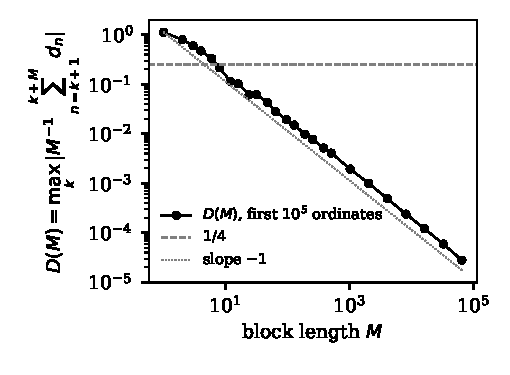
\includegraphics[width=0.48\textwidth]{figures/fig_blockmeans.pdf}\hfill
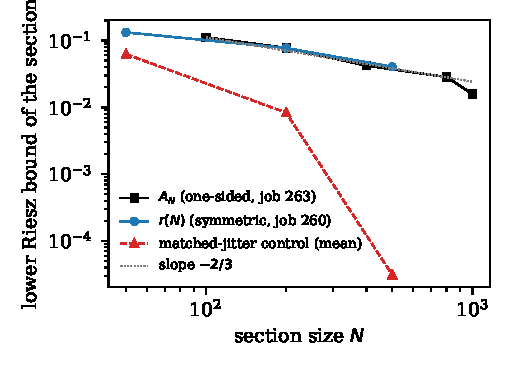
\includegraphics[width=0.48\textwidth]{figures/fig_riesz.pdf}
\caption{Left: $D(M)$ against $M$ over the first $10^5$ ordinates, with the $\frac14$ line and a reference slope $-1$. Right: lower Riesz constants of finite sections: $A_N$ for the one-sided sections $\{x_n\}_{n\le N}$ (job 263), $r(N)$ for the symmetric sections $\{\pm x_n\}_{n\le N}$ (job 260), the mean over $100$ draws of the matched sup-norm jitter control, and a reference slope $-2/3$.}\label{fig:D}
\end{figure}

\paragraph{Finite sections.} For the one-sided sections at $N=100,200,400,800,1000$ the lower constants are $A_N=0.1115$, $0.0774$, $0.0421$, $0.0283$, $0.0159$ and the upper constants $B_N=1.953$, $2.062$, $2.115$, $2.277$, $2.278$, computed at $50$ digits (job 263; the recorded eigenpair residuals are below $8.4\cdot10^{-31}$ in the job's primary normalization and below $1.4\cdot10^{-30}$ for eigenvectors normalized in the sup norm). The closest pair among the first $1000$ has gap $s_{1000}=0.1376$ and Proposition~\ref{prop:finite} gives $A_{1000}\le1-\sinc(0.1376)=0.0309$; among the first $10^5$ the closest pair has gap $0.02186$ (at $n=95248$, $\gamma\approx71732.9$, the Lehmer-type pair with ordinate gap $0.0147$), which forces $A_{10^5}\le7.9\cdot10^{-4}$. For the symmetric sections $\{\pm x_n\}_{n\le N}$ of $\Lam_{3/2}$ (without the point $0$; finite sections cannot see the missing point, since sections of $\Z\setminus\{0\}$ and of $\Z$ are both orthogonal) $r(N)=0.1324$, $0.0771$, $0.0404$ at $N=50,200,500$, computed at $60$ digits; a control ensemble of $100$ sequences $n+u_n$ with $u_n$ uniform on $[-\max_{n\le N}|d_n|,\max_{n\le N}|d_n|]$ has mean $r$ equal to $0.0625$, $0.0083$, $3.1\cdot10^{-5}$ (job 260), so the arithmetic ordinates keep a lower bound three orders of magnitude above matched random jitter at $N=500$. The jitter ensemble matches the largest displacement only (at $N=500$ its root-mean-square displacement is $0.38$, against $0.25$ for the zeros), and its points are independent, so neighbors can nearly collide; it is not the random-matrix model of the zeros, and a comparison with sections of the sine process is not carried out here. The upper constants grow slowly; whether they stay bounded is the Bessel half of the frame question of Section~\ref{sec:open}, which also asks for a lower frame bound and completeness.

\section{Provenance}\label{sec:provenance}

The harness record posed the fixed-block question answered by Theorem~\ref{thm:kadec} and the Riesz-basis question answered by Theorem~\ref{thm:main}. Hypnos~\cite{HypnosMethods} is a research harness built at the direction of David Ross. Its proposal models are Gemma~4 31B, a dense model in 4-bit activation-aware weight quantization (AWQ), \path{QuantTrio/gemma-4-31B-it-AWQ}; Gemma~4 26B, a mixture-of-experts model with 4 billion active parameters, served in AWQ from a quantization of \path{google/gemma-4-26B-A4B-it}; and Qwen3 32B, a dense model in 4-bit AWQ, \path{Qwen/Qwen3-32B-AWQ}. They run through vLLM on hardware operated by Ross and generate mathematical claims from a notebook of structured records. Claude Opus (Anthropic), accessed through a subscription, reviews samples under pre-registered rules; claims selected for execution include a computation that the harness runs against its verification routines. Proposals, verdicts and execution records are retained in the private repository and database. The site \url{https://hypnosmath.org} publishes reviewed explanations and selected computational records. Between 12 August and 27 September 2026 the harness generated the line of questions studied here: whether the unfolded ordinates are a Kadec-admissible perturbation of the integers (its node 537, run 3), the recognition that the Kadec quantity is a bound on $S$ at the ordinates and that a centering convention was contaminating the numbers (nodes 831, 1540, 2059, 2371), the passage to Avdonin's averaged condition (nodes 1032, 1034, 1115, 1870, 2057, 2393, 2400), the conjectures that the Kadec failure is unconditional and shift-invariant (nodes 1296, 1637, 1638), and the replacement of the yes-or-no sufficient conditions by measured Riesz constants of finite sections (nodes 1687, 2181). Its execution tier produced the measurements of Section~\ref{sec:numerics} (jobs 25, 48, 67, 100, 110, 166, 202, 260, 263, 313; their records are in the project's private repository, jobs 25 and 48 through their recorded check values, since their artifact directories were not retained). A literature sweep run by the harness on 28 August 2026 found no treatment of the zeta ordinates as a frame, Riesz basis, or Kadec object in print. Two works are adjacent. Mikulik \cite{Mikulik}, a preprint of April 2026 of which we have seen only the abstract, unfolds the ordinates to unit mean spacing, studies Gaussian Gram matrices of local clusters, derives a Fourier representation through nonharmonic exponential systems, and conjectures a uniform lower bound on the minimal eigenvalue, a frame inequality of a different kind from the fixed-interval Riesz-basis question treated here. Burnol \cite{Burnol04} constructs complete and minimal systems attached to the zeros in de Branges' Sonine spaces, not the exponential family on a bounded interval. Neither accessible account states Theorem~\ref{thm:main}, and we have not checked Mikulik's full manuscript; our own searches for the ordinates as a frame, Riesz basis, complete interpolating sequence, or Kadec object found no earlier proof of it; that is a bounded search, not a certification of priority.

Claude Fable 5.1 developed the proofs while writing this manuscript. Theorem~\ref{thm:identity} formalizes what the harness had measured; Theorem~\ref{thm:kadec} answers the question its nodes 1870 and 2400 asked, namely whether Avdonin's mean condition survives where Kadec's fails (it does not, for any fixed block length; below height $T$ it does at block lengths of order $\log^2T$, Corollary~\ref{cor:growing}); Theorem~\ref{thm:main} answers the question of nodes 1687 and 2181, whether the Riesz property degrades or is merely uncertified (it is lost). David Ross directed the work and takes responsibility for its communication. The proofs use the classical results cited in Section~\ref{sec:inputs} and, for the lower bound in Theorem~\ref{thm:BM}(a), Conrey's theorem \cite{Conrey89}; the harness supplied the motivating questions and the numerical observations, which are reported separately from the proofs.

\subsection*{Data and code}
Published with this paper at \url{https://hypnosmath.org/research/unfolded-zeros-not-a-riesz-basis}, where the page links each file: the verification script for Theorem~\ref{thm:identity}, Proposition~\ref{prop:block} and the Kadec and Avdonin statistics over the first $10^4$ ordinates (\texttt{verify\_identity.py}); the recomputation over all $10^5$ (\texttt{verify\_kadec\_1e5.py}); and the recorded outputs of both (\texttt{verify\_10000.json} and \texttt{verify\_10000\_40samples.json}, the $12$- and $40$-sample identity runs over the first $10^4$ ordinates; \texttt{verify\_kadec\_1e5.json}, the Kadec and Avdonin run over all $10^5$). Held in the project's private repository and not published: the figure script; the harness's records for the ten jobs cited above (the result and artifact files of jobs 67, 100, 110, 166, 202, 260, 263 and 313, and for jobs 25 and 48 the execution records with their check values, copied from the harness's database); and the table of the first $10^5$ ordinates that both scripts read, computed by the harness to $200$ significant digits and checked against the published counting function, so the published files alone do not rerun the computations.

\begin{thebibliography}{99}

\bibitem{AlemanyNitzan} T.~Alemany and S.~Nitzan, On the lower Riesz basis bound of exponential systems over an interval, arXiv:2501.11598 (2025).

\bibitem{AlpogeFurman} L.~Alp\"oge and R.~Furman, More than two thirds of the zeta zeros are simple and on the critical line, arXiv:2608.13637 (2026).

\bibitem{Avdonin74} S.~A.~Avdonin, On the question of Riesz bases of exponential functions in $L^2$, Vestnik Leningrad. Univ. No.~13 (1974), 5--12; English transl. Vestnik Leningrad Univ. Math. 7 (1979), 203--211.

\bibitem{BM67} A.~Beurling and P.~Malliavin, On the closure of characters and the zeros of entire functions, Acta Math. 118 (1967), 79--93.

\bibitem{Bober} J.~W.~Bober and G.~A.~Hiary, New computations of the Riemann zeta function on the critical line, Exp. Math. 27 (2018), 125--137.

\bibitem{Bufetov} A.~I.~Bufetov, The sine-process has excess one, arXiv:1912.13454 (2019).

\bibitem{Burnol04} J.-F.~Burnol, Two complete and minimal systems associated with the zeros of the Riemann zeta function, J. Th\'eor. Nombres Bordeaux 16 (2004), 65--94.

\bibitem{Conrey89} J.~B.~Conrey, More than two fifths of the zeros of the Riemann zeta function are on the critical line, J. Reine Angew. Math. 399 (1989), 1--26.

\bibitem{Dyson} F.~J.~Dyson and M.~L.~Mehta, Statistical theory of the energy levels of complex systems IV, J. Math. Phys. 4 (1963), 701--712.

\bibitem{Ghosh} S.~Ghosh, Determinantal processes and completeness of random exponentials: the critical case, Probab. Theory Related Fields 163 (2015), 643--665.

\bibitem{GoldstonGonek} D.~A.~Goldston and S.~M.~Gonek, A note on $S(t)$ and the zeros of the Riemann zeta-function, Bull. London Math. Soc. 39 (2007), 482--486.

\bibitem{HNP} S.~V.~Hru\v{s}\v{c}ev, N.~K.~Nikol'skii and B.~S.~Pavlov, Unconditional bases of exponentials and of reproducing kernels, in: Complex Analysis and Spectral Theory, Lecture Notes in Math. 864, Springer, Berlin, 1981, 214--335.

\bibitem{HypnosMethods} Claude Fable 5, at the direction of D.~Ross, Self-grading without self-deception: verdict discipline for a long-running mathematical research agent, manuscript (August 2026), Hypnos Math, \url{https://hypnosmath.org}.

\bibitem{Inoue26} S.~Inoue, Small gaps between consecutive zeros of the Riemann zeta-function, arXiv:2604.05733 (2026).

\bibitem{JohnNirenberg} F.~John and L.~Nirenberg, On functions of bounded mean oscillation, Comm. Pure Appl. Math. 14 (1961), 415--426.

\bibitem{Kadec64} M.~I.~Kadec, The exact value of the Paley--Wiener constant, Dokl. Akad. Nauk SSSR 155 (1964), 1253--1254; Soviet Math. Dokl. 5 (1964), 559--561.

\bibitem{KoosisII} P.~Koosis, The Logarithmic Integral II, Cambridge Stud. Adv. Math. 21, Cambridge Univ. Press, 1992.

\bibitem{KozmaLev} G.~Kozma and N.~Lev, Exponential Riesz bases, discrepancy of irrational rotations and BMO, J. Fourier Anal. Appl. 17 (2011), 879--898.

\bibitem{Landau67} H.~J.~Landau, Necessary density conditions for sampling and interpolation of certain entire functions, Acta Math. 117 (1967), 37--52.

\bibitem{Littlewood24} J.~E.~Littlewood, On the zeros of the Riemann zeta-function, Proc. Cambridge Philos. Soc. 22 (1924), 295--318.

\bibitem{LyubarskiiSeip} Yu.~I.~Lyubarskii and K.~Seip, Complete interpolating sequences for Paley--Wiener spaces and Muckenhoupt's $(A_p)$ condition, Rev. Mat. Iberoamericana 13 (1997), 361--376.

\bibitem{Mikulik} J.~Mikulik, Unfolded Gaussian Gram stability for zeta zeros, preprint, April 2026. ResearchGate publication 403995908, \url{https://www.researchgate.net/publication/403995908}.

\bibitem{Pavlov79} B.~S.~Pavlov, Basicity of an exponential system and Muckenhoupt's condition, Dokl. Akad. Nauk SSSR 247 (1979), 37--40; Soviet Math. Dokl. 20 (1979), 655--659.

\bibitem{PRZZ} K.~Pratt, N.~Robles, A.~Zaharescu and D.~Zeindler, More than five-twelfths of the zeros of $\zeta$ are on the critical line, Res. Math. Sci. 7 (2020), Paper No.~2, doi:10.1007/s40687-019-0199-8.

\bibitem{SeipUlanovskii} K.~Seip and A.~M.~Ulanovskii, The Beurling--Malliavin density of a random sequence, Proc. Amer. Math. Soc. 125 (1997), 1745--1749.

\bibitem{Selberg46} A.~Selberg, Contributions to the theory of the Riemann zeta-function, Arch. Math. Naturvid. 48 (1946), 89--155.

\bibitem{Selberg46b} A.~Selberg, Contributions to the theory of Dirichlet's $L$-functions, Skr. Norske Vid.-Akad. Oslo I (1946), no.~3, 1--62.

\bibitem{Selberg92} A.~Selberg, Old and new conjectures and results about a class of Dirichlet series, in: Proceedings of the Amalfi Conference on Analytic Number Theory (Maiori, 1989), Univ. Salerno, 1992, 367--385.

\bibitem{Titchmarsh} E.~C.~Titchmarsh, The Theory of the Riemann Zeta-Function, 2nd ed., revised by D.~R.~Heath-Brown, Oxford Univ. Press, 1986.

\bibitem{Tsang86} K.-M.~Tsang, Some $\Omega$-theorems for the Riemann zeta-function, Acta Arith. 46 (1986), 369--395.

\end{thebibliography}

\end{document}
